\documentclass[11pt]{article}

% ------------------------------------------------------------------------------
% This is all preamble stuff that you don't have to worry about.
% Head down to where it says "Start here"
% ------------------------------------------------------------------------------

\usepackage[margin=.8in,top=1.1in,bottom=1.1in]{geometry} % page layout
\usepackage{amsmath,amsthm,amssymb,amsfonts} % math things
\usepackage{graphicx} % include graphics
\usepackage{fancyhdr} % header customization
\usepackage{titlesec} % help with section naming
\usepackage{listings}
\usepackage[final]{pdfpages}
\usepackage{pgfplots}
\usepackage{float}

\pgfplotsset{compat=1.7}

% naming sections
\titleformat{\section}{\bf}{Problem \thesection}{0.5em}{}
\newcommand{\exercise}{\section{}}

% headers
\pagestyle{fancy}
\fancyhf{} % clear all
\fancyhead[L]{\sffamily\small Machine Learning 1 --- Homework}
\fancyhead[R]{\sffamily\small Page \thepage}
\renewcommand{\headrulewidth}{0.2pt}
\renewcommand{\footrulewidth}{0.2pt}
\markright{\hrulefill\quad}

\newcommand{\hwhead}[4]{
\begin{center}
\sffamily\large\bfseries Machine Learning Worksheet #1
\vspace{2mm}
\normalfont

#2\\
#3\\
\texttt{#4}
\end{center}
\vspace{6mm} \hrule \vspace{4mm}
}

% ------------------------------------------------------------------------------
% Start here -- Fill in your name, imat and email
% (and the same for who you worked with)
% You are allowed to work in groups of 2 (or 3 if there is no way around it)
% However, you each must submit individually - (it may be same file)
% ------------------------------------------------------------------------------

\newcommand{\names}{Tomas Ladek, Michael Kratzer} %
\newcommand{\imats}{3602673, 3612903} %
\newcommand{\emails}{tom.ladek@tum.de, mkratzer@mytum.de} %

\begin{document}

% ------------------------------------------------------------------------------
% Change xx (and only xx) to the current sheet number
% ------------------------------------------------------------------------------
\hwhead{7}{\names}{\imats}{\emails}

% ------------------------------------------------------------------------------
% Fill in your solutions
% ------------------------------------------------------------------------------

\exercise
Let us rewrite the sigmoid activation function as
\begin{align*}
	\sigma(x) &= \dfrac{1}{1 + e^{-x}} = \dfrac{e^x}{e^x (1 + e^{-x})} = \dfrac{e^x}{e^x + e^{x-x}} = \dfrac{e^x}{e^x + 1}
\end{align*}
There exists a network that computes $\sigma(x)$ by scaling and offsetting the hyperbolic tangent function $\tanh(x)$, since
\begin{align*}
	\tanh(x) &= \dfrac{e^x - e^{-x}}{e^x + e^{-x}} \\
	&= \dfrac{e^{-x} (e^{2x} - 1)}{e^{-x} (e^{2x} + 1)} \\
	&= \dfrac{e^{2x} - 1}{e^{2x} + 1} \\
	&= \dfrac{2e^{2x} - (1 + e^{2x})}{e^{2x} + 1} \\
	&= \dfrac{2e^{2x}}{e^{2x} + 1} - \dfrac{1 + e^{2x}}{e^{2x} + 1}\\
	&= 2 \dfrac{e^{2x}}{e^{2x} + 1} - 1\\
	&= 2 \sigma(2x) - 1
\end{align*}
And therefore
\begin{align*}
	\tanh(x) &= 2 \sigma(2x) - 1\\
	\tanh(x) + 1 &= 2 \sigma(2x)\\
	\dfrac{1}{2} (\tanh(x) + 1) &= \sigma(2x)\\
	\dfrac{1}{2} (\tanh(\dfrac{z}{2}) + 1) &= \sigma(z) \quad\quad with\ z = 2x	
\end{align*}

\exercise
\begin{align*}
	\dfrac{d}{dx}\ \sigma(x) = \dfrac{d}{dx}\ \dfrac{e^x}{e^x + 1} &= \dfrac{(e^x + 1) e^x - e^x e^x}{(e^x + 1)^2}\\
	&= \dfrac{(e^{x} + 1)e^x}{(e^x + 1)^2} - \dfrac{(e^{x})^2}{(e^x + 1)^2}\\
	&= \dfrac{e^x}{e^x + 1} - \Big(\dfrac{e^x}{e^x + 1}\Big)^2\\
	&= \sigma(x) - \sigma^2(x)
\end{align*}

\begin{align*}
	\dfrac{d}{dx}\ \tanh(x) &= \dfrac{d}{dx}\ \dfrac{e^x - e^{-x}}{e^x + e^{-x}} 
	= \dfrac{(e^x + e^{-x})(e^x + e^{-x}) - (e^x - e^{-x})(e^x - e^{-x})}{(e^x + e^{-x})^2}\\
	&= \dfrac{(e^x + e^{-x})^2 - (e^x - e^{-x})^2}{(e^x + e^{-x})^2} = 1 - \Big(\dfrac{e^x - e^{-x}}{e^x + e^{-x}}\Big)^2 = 1 - \tanh^2(x)
\end{align*}

\exercise
\#trivial

\exercise
\#trivial

\exercise
Below six plots of the training curves for different learning rates used in \texttt{mlp\_xor.NeuralNetwork(X,y,l)} and \texttt{mlp\_sin.NeuralNetwork(X,y,l)} respectively.
\section*{mlp\_xor.NeuralNetwork(X,y,l):}
\begin{figure}[H]
	\centering
	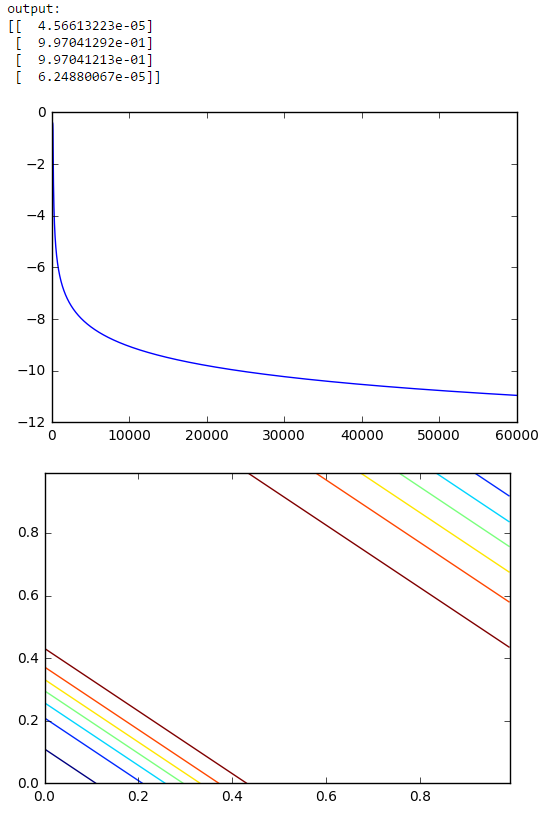
\includegraphics[width=0.7\linewidth]{xor_lr03}
	\caption{Function: XOR, Learning rate 0.3}
	\label{fig:xorlr03}
\end{figure}
\begin{figure}[H]
	\centering
	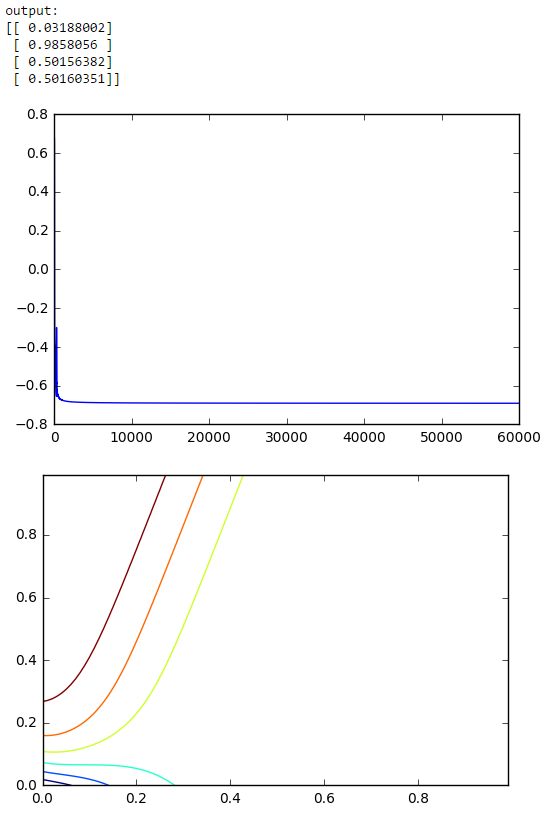
\includegraphics[width=0.7\linewidth]{xor_lr06}
	\caption{Function: XOR, Learning rate 0.6}
	\label{fig:xorlr06}
\end{figure}
\begin{figure}[H]
	\centering
	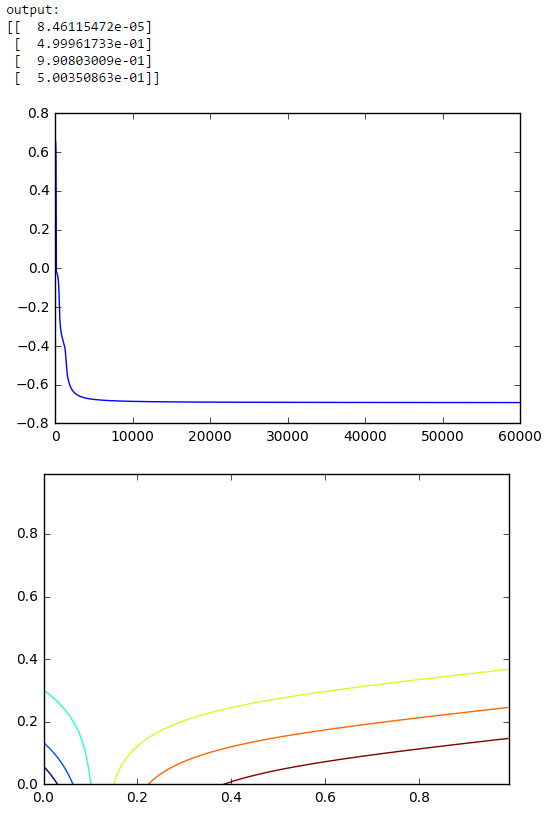
\includegraphics[width=0.7\linewidth]{xor_lr005}
	\caption{Function: XOR, Learning rate 0.05}
	\label{fig:xorlr005}
\end{figure}

\section*{mlp\_sin.NeuralNetwork(X,y,l):}
\begin{figure}[H]
	\centering
	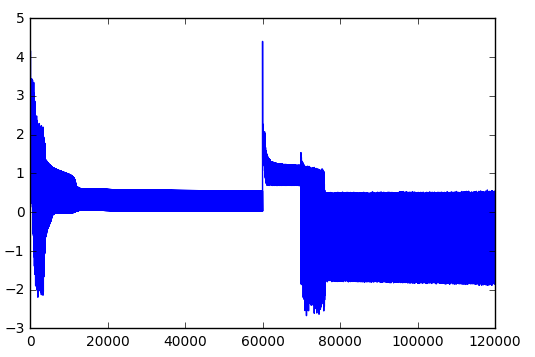
\includegraphics[width=0.7\linewidth]{sin_lr03}
	\caption{Function: Sin, Learning rate 0.3}
	\label{fig:sinlr03}
\end{figure}
\begin{figure}[H]
	\centering
	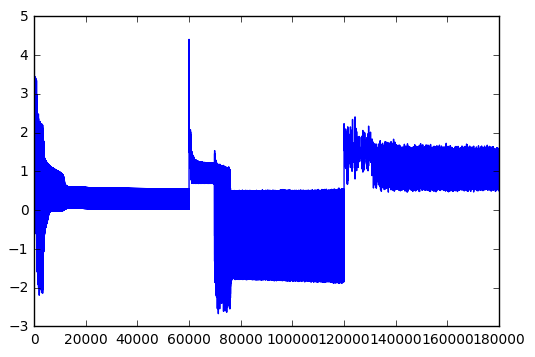
\includegraphics[width=0.7\linewidth]{sin_lr07}
	\caption{Function: Sin, Learning rate 0.7}
	\label{fig:sinlr07}
\end{figure}
\begin{figure}[H]
	\centering
	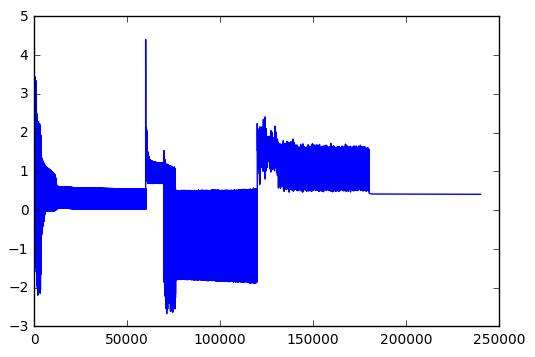
\includegraphics[width=0.7\linewidth]{sin_lr005}
	\caption{Function: Sin, Learning rate 0.05}
	\label{fig:sinlr005}
\end{figure}

\exercise
\#goodquestion

\exercise
\#goodquestion

\end{document}